% !TeX root = Protokoll.tex
\subsection{Versuchsaufbau}
\begin{figure}
	\centering
	\begin{tikzpicture}
			
			\node [draw=white, anchor=south west] (label) at (0,0) {
				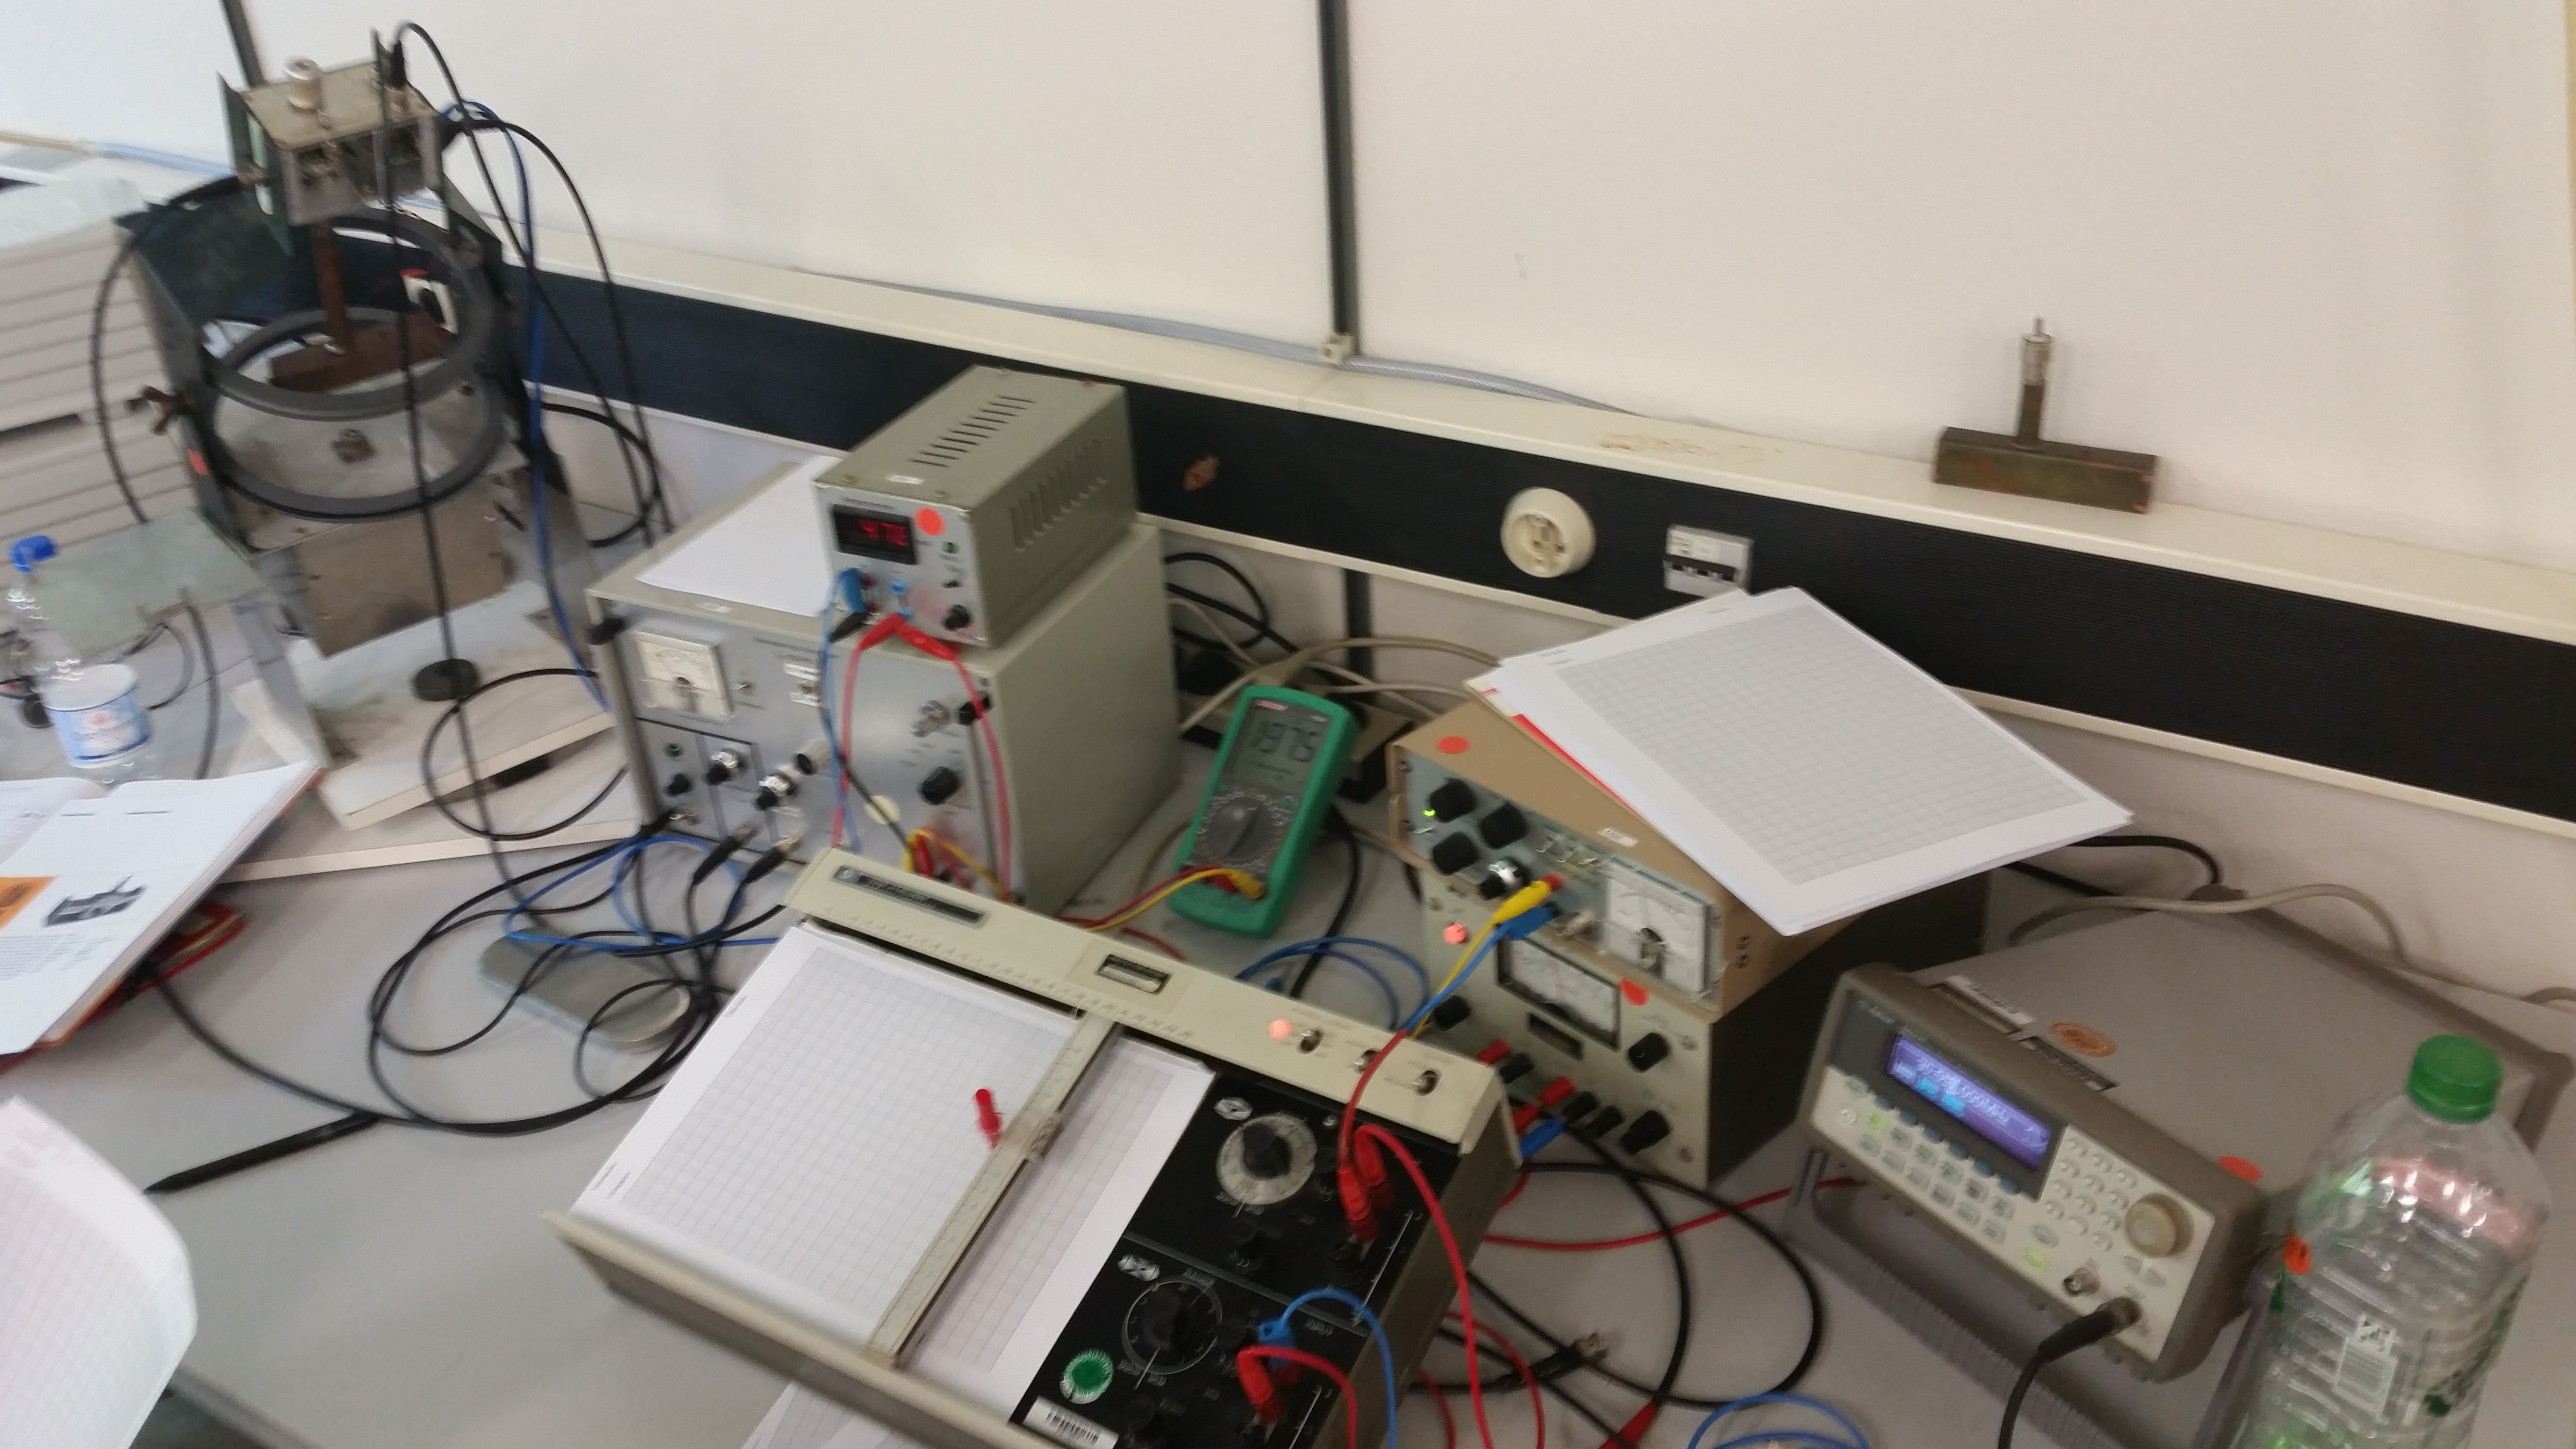
\includegraphics[width=1.0\textwidth]{../Grafiken/Aufbau.jpg}};
%			\draw[step=.5cm,draw=gray] (0.0,0.0) grid (\textwidth,\textwidth - 180);
%			\foreach \x in {0,1,...,16}
%				\filldraw [fill=green] (\x,0) node[below] {\x};
%			\foreach \y in {0,1,...,10}
%				\filldraw [fill=green] (0,\y) node[left] {\y};
				
			\draw [very thick] (2.0,8.5) -- (1.0,8.5);
			\node [draw=black,shape=circle,fill=lightgray] (1.) at (1.0,8.5) {1};
			\draw [very thick] (3.0,7.5) -- (4.0,7.5);
			\node [draw=black,shape=circle,fill=lightgray] (1.) at (4.0,7.5) {2};
			\draw [very thick] (2.25,6.85) -- (1.0,6.85);
			\node [draw=black,shape=circle,fill=lightgray] (1.) at (1.0,7.0) {3};
			\draw [very thick] (5.0,5.5) -- (5.0,6.5);
			\node [draw=black,shape=circle,fill=lightgray] (1.) at (5.0,6.5) {4};
			\draw [very thick] (6.0,6.5) -- (6.0,7.5);
			\node [draw=black,shape=circle,fill=lightgray] (1.) at (6.0,7.5) {5};
			\draw [very thick] (8.0,4.5) -- (8.0,5.5);
			\node [draw=black,shape=circle,fill=lightgray] (1.) at (8.0,5.5) {6};
			\draw [very thick] (7.0,3.0) -- (7.0,4.0);
			\node [draw=black,shape=circle,fill=lightgray] (1.) at (7.0,4.0) {7};
			\draw [very thick] (9.5,4.5) -- (9.5,5.5);
			\node [draw=black,shape=circle,fill=lightgray] (1.) at (9.5,5.5) {8};
			\draw [very thick] (10.5,2.) -- (10.5,1.);
			\node [draw=black,shape=circle,fill=lightgray] (1.) at (10.5,1.) {9};
			\draw [very thick] (13,2.5) -- (13.,3.5);
			\node [draw=black,shape=circle,fill=lightgray] (1.) at (13.,3.5) {10};						

		\end{tikzpicture}
			\caption{Der verwendete Versuchsaufbau zur Durchführung von ESR-Messung}\label{fig:Aufbau}
\end{figure}

Der im Folgenden beschriebene Versuchsaufbau ist in \cref{fig:Aufbau} dargestellt.
Die zu untersuchende Probe (3) ist innerhalb einer Helmholtz-Spule (2) befestigt. Dabei wurde die Helmholtz-Spule so 
ausgerichtet das sie parallel beziehungsweise antiparallel zum Erdmagnetfeld ist, da dieses die durchzuführende 
Messung beeinflusst. Durch jeweils zwei Messungen, von denen die Eine in paralleler und die Andere in antiparalleler Ausrichtung der Magnetfelder durchgeführt wird, kann die Größe des Erdmagnetfeldes bestimmt und dessen Einfluss auf die Messung herausgerechnet werden.
Betrieben wird die Helmholtz-Spule unter Verwendung eines Rampengenerators (8) und eines Leistungsverstärkers (9). Mittels Rampengenerator
wird eine zeitproportionale Dreiecksspannung erzeugt, die verwendet wird, um über den Leistungsverstärker einen zu dieser proportionalen Strom
zu erzeugen. Dieser Storm wird zum Betrieb der der Helmholtz-Spulen verwendet. Es wird eine Dreieckspannung verwendet, um sowohl negative 
als auch positive, linear von der Zeit abhängige, Ströme zu erzeugen und so beide Magnetfeldausrichtungen messen zu können ohne die 
Spulenausrichtung zu verändern. Die Stromstärke die an den Helmholtz-Spulen anliegt, kann an einem Amperemeter (5) abgelesen werden,
um die aufzunehmende Resonanzkurve zu kalibrieren.

Die Probe befindet sich ferner in einer HF-Spule, die an die Brückenschaltung (1 / 4) angeschlossen ist. Durch Abgleichen der Brückenschaltung 
vor dem Anstellen des Magnetfeldes, können so kleinste Veränderungen des komplexen Widerstands der HF-Spule gemessen werden. Diese Änderungen 
werden durch die in der Probe induzierte Magnetisierung hervorgerufen.
Betrieben wird die HF-Spule unter Verwendung eines Hochfrequenz-Generators (10). 

Ein Überlagerungsempfänger (4) ist der Brückenschaltung (4) nachgeschaltet, dieser wird
dafür eingesetzt, die Brückenspannung von Störspannungen zu trennen. Zur Verstärkung der zu messenden Spannung wird ein ZF-Verstärker (4)
verwendet. Für die Verwendung eines solchen Selektivverstärkers, wird die zu verstärkende Spannung zunächst mit einer Spannung der Frequenz 
$f_{\text{OSZ}}$, eines zusätzlichen Oszillators überlagert. Die Frequenz $f_{\text{OSZ}}$ wird so gewählt, dass die entstehende 
Schwebungsfrequenz der Frequenz $f_{\text{ZF}}$ entspricht, die von dem ZF-Verstärker verstärkt wird. Durch anschließende Demodulation der so 
verstärkten und von Störungen getrennten 
Spannung, ergibt sich die verstärkte Brückenspannung, die mit Hilfe eines Multimeters (6) gemessen werden. Dieses
Messinstrument kann sowohl dazu verwendet werden die Brücke auf Null abzugleichen als auch dazu im Verlauf der Brückenspannung Extrema erkennen zu können.

Diese Resonanzkurven werden unter Verwendung eines XY-Schreibers (7) aufgenommen. 
Die Auslenkung in $x$-Richtung ist dabei proportional zu der Spannung des Rampengenerators, währende die Auslenkung in $y$-Richtung  
proportional zur verstärkten Brückenspannung ist.     
 
%Um die Probe ist noch eine kleinere Spule die an eine Brückenschaltung (3) angeschlossen ist, diese Spule wird durch einen Hochfrequenz-Generator betrieben (9), in der Brückenschaltung ist noch ein Empfänger eingebaut mithilfe das Signal von Störungen getrennt werden kann.
%Rechts neben der Brückenschaltung ist ein Multimeter (5) mit dem die Spannung der Brückenschaltung gemessen werden kann.
%Rechts davon ist der Rampengenerator (7) zusehen mit dem die Helmholtz-Spule betrieben wird.
%Im Vordergrund ist ein XY-Schreiber (6) zu sehen wo die Spannung der Brückenschaltung und des Rampengenerator angelegt werden.
%Die Stromstärke an der Helmholtz-Spule kann mit einem Ampere Meter gemessen werden (4).
\subsection{Messverfahren}
%An der Brückenschaltung können die Frequenzen $\nu_\text{Osz}$ und $\nu_\text{ZF}$ eingestellt werden, mit diesen beiden Frequenzen kann das 
%Störsignal verringert werden und das Signal der Elektronen $\nu_e$ ausgefiltert werden. Dabei gilt
Zunächst wird eine der möglichen Oszillatorfrequenz $f_{\text{OSZ}}$ eingestellt und die Frequenz des HF-Generators so gewählt, dass diese
die Bedingung in \cref{eq:Freq_Bedinung} erfüllen.  
\begin{align}
\label{eq:Freq_Bedinung}
f_{\text{HF}}=f_{\text{ZF}}+f_{\text{OSZ}}.
\end{align}
Vor dem Anstellen des Magnetfeldes wird die Brückenspannung mit Hilfe der Stellglieder $R$, $C_{\text{grob}}$ und $C_{\text{fein}}$ 
zunächst auf Null abgestimmt, um diese infolgedessen, unter Verwendung von $R$, leicht zu verstimmen. Durch Einschalten des Rampengenerators
wird von den Helmholtz-Spulen ein mit der Zeit anwachsendes Magentfeld erzeugt. Kann bei Betrachtung des Multimeters ein Extremum in der 
Brückenspannung festgestellt werden, wird die Veränderung der Brückenspannung in Abhängigkeit
der Rampengeneratorspannung mit dem XY-Schreiber aufgenommen. Die so aufgenommenen Resonanzkurven sollten der Form nach den in 
\cref{fig:Resonanz} dargestellten Kurven entsprechen.    
%dies ist die Frequenz die am Hochfrequenz-Generator eingestellt werden sollte.
%Bei abgestellten Magnetfeld der Helmholtz-Spule wird eine die minimale Brückenspannung eingestellt, indem der Kondensator $C$ und der Wiederstand $R$, der Brückenschaltung verstellt werden, dann wird das Signal mithilfe des Verstärkers auf ein Maximum verstärkt.\\
%Nun wird der mithilfe des Rampengenerators eine Sägezahnspannung an die Helmholtz-Spule angelegt.
%Im Spannungsverlauf der Brückenschaltung sollte ein globales Maximum oder ein globales Minimum zu sehen sein (\cref{fig:Resonanz}). 
%Kann sowohl ein Maxima als auch ein Minimum zu erkennt werden, liegt eine Überlagerung der beiden Kurven vor.
%Dies Geschieht dadurch das $C$ an der Brückenschaltung verstimmt ist.
% Dies kann durch feines verstellen der Brücke ausgeglichen werden.
\begin{wrapfigure}{r}{0.5\textwidth}
\centering
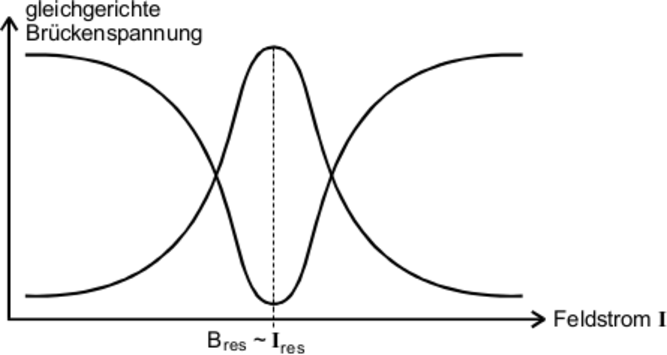
\includegraphics[width=0.5\textwidth]{../Grafiken/Resonanz.pdf}
\caption{Darstellung von zwei möglichen Resonanzkurven, die mit dem XY-Schreiber aufzunehmen sinds.\cite{V28}}\label{fig:Resonanz}
\end{wrapfigure}

Da aus der Resonanzkurve der Strom $I_{\text{res}}$ und aus diesem das Magnetfeld  
$B_{\text{res}}$ an der Resonanzstelle bestimmt werden soll, ist eine Kalibration der $x$-Achse des XY-Schreibers notwendig. Diese wird 
durchgeführt, indem Minimum und Maximum des Spulenstroms den entsprechenden Start und Endpunkten der Resonanzkurve zugeordnet werden. 
Mit dem Abstand dieser Punkte auf dem Millimeterpapier kann die $x$-Achse auf die Stromstärke kalibriert werden. Dieses Vorgehen ist 
beispielhaft in \cref{fig:resonanzkurve_20555+_cut} gezeigt. Aus den so bestimmten Strömen $I_{\text{res}}$ kann 
die magnetische Feldstärke der Helmholtz-Spule mit der Windungszahl $N$ und
dem Spulenradius $R$ nach \cref{eq:helmholtz}\,\cite{V28} bestimmt werden.
\begin{empheq}{equation}
	B(I) = \dfrac{8\cdot \mu_0}{\sqrt{125}} \cdot \dfrac{I_{\text{res}}\cdot N}{R}
	\label{eq:helmholtz}
\end{empheq}
